\chapter{Particle system}
\label{cha:particlesystem}

Particle system is one of most commonly used techniques to simulate smoke, fire, rain and other groups of discrete objects, usually independent from each other. System consist of defined number of emitters, producing lightweight particle objects with certain parameters. Each emitter has defined production ratio and each particle a certain lifespan, resulting in upper limit of total particles on screen. Some systems use also attraction points which enable better control over particles, using equations often similar to those of electrostatic forces.
Such simulation is independent from rendering. The same particle system may be used for different effects with proper configuration.

\begin{figure}[h!]
  \caption{Example rendering of tested particle system}
  \label{img:particles}
  \centering
	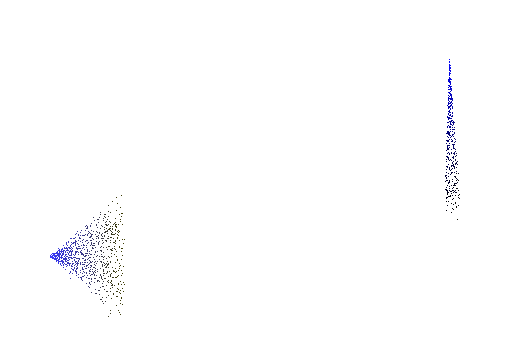
\includegraphics[width=16cm]{particles}
\end{figure}

\section{System parameters}
\label{sec:emittersparameters}

Tested system works on two-dimensional Cartesian plane. For purpose of  performance analysis movements are calculated based only on frames rather than actual flow of time. This means that systems with different framerate will result in different visualisations, but requesting given amount of frames rendered will result in the same lifespan and total number of particles in both systems.

Emitter supports following parameters:

\begin{itemize}
	\item position - initial position of created particles
	\item angle - angle counting clockwise from vector [0, 1]
	\item spread - parameter controlling random differences in initial angle of particles
	\item velocity - initial velocity of particles, in pixels per frame
	\item velocity spread - parameter controlling random differences in initial velocity of particles
	\item lifespan - initial lifespan of particles
	\item productionRate - amount of particles initialized in each frame
\end{itemize}

A Particle has similar properties:
\begin{itemize}
	\item position
	\item velocity
	\item lifespan
	\item age - counted in frames, when higher then lifespan particle is removed from system
\end{itemize}

Source code of both implementations is attached in Appendix \ref{cha:sourcecode}.

\section{Implementation with high memory allocation}
\label{sec:particlesinitial}

Initial tested implementation has one very important property of particle emitter. Whenever new particles are created, new array of pointers is allocated and returned from emitter. System appends new particles to existing array. In each frame particle system creates new, empty array of particles and adds there only particles that are still alive. Array from previous frame and all dead particles are removed from system and deallocated. This is clearly suboptimal solution that allocates and deallocates plenty of memory in each frame. Purpose of this exercise is to show how both languages handle bad code and how big impact it has comparing to the optimal solution.

TODO: this part may need to be updated before publication.
TODO: Is this accounting properly for v8 startup time? Maybe profiling ticks would be better.

\lstinputlisting[caption=Time measurement of unoptimized particle system in JavaScript,label=listing:timejs1]{particles/timejs1.txt}
\lstinputlisting[caption=Time measurement of unoptimized particle system in C++,label=listing:timecpp1]{particles/timecpp1.txt}

Time measurement shows that JavaScript version is almost 8 times slower than native one. To analyse situation --prof and --log-timer-events flags may be used. Output file v8.log is parsed using available online tool.\footnote{http://v8.googlecode.com/svn/branches/bleeding\_edge/tools/profviz/profviz.html}

\lstinputlisting[caption=Profiler output for unoptimized particles,label=listing:particles1profile]{particles/particles1-profile.txt}

Methods prefixed with ~ are unoptimized, the ones prefixed with * are JIT compiled. As seen in profiler log, most of the time is spent in unoptimised versions of verifyIfAlive and stepParticle methods of particle system step.

\lstinputlisting[caption=Annotated part of source,label=listing:particles1stepannotated,language=JavaScript]{particles/particleSystemStep.js}

The same methods are also used in optimised versions, where they take significantly less ticks to run. It's clear that presented code not only allocates and deallocates too much memory, but also fails to run in optimised mode. It's visible on chart obtained from the same tool - stripe labelled "code kind in execution" shows multiple kinds of code running and is interrupted often with garbage collection cycles.

\begin{figure}[h!]
  \caption{Chart of time used in unoptimised verion of JavaScript}
  \label{img:particles1profile}
  \centering
	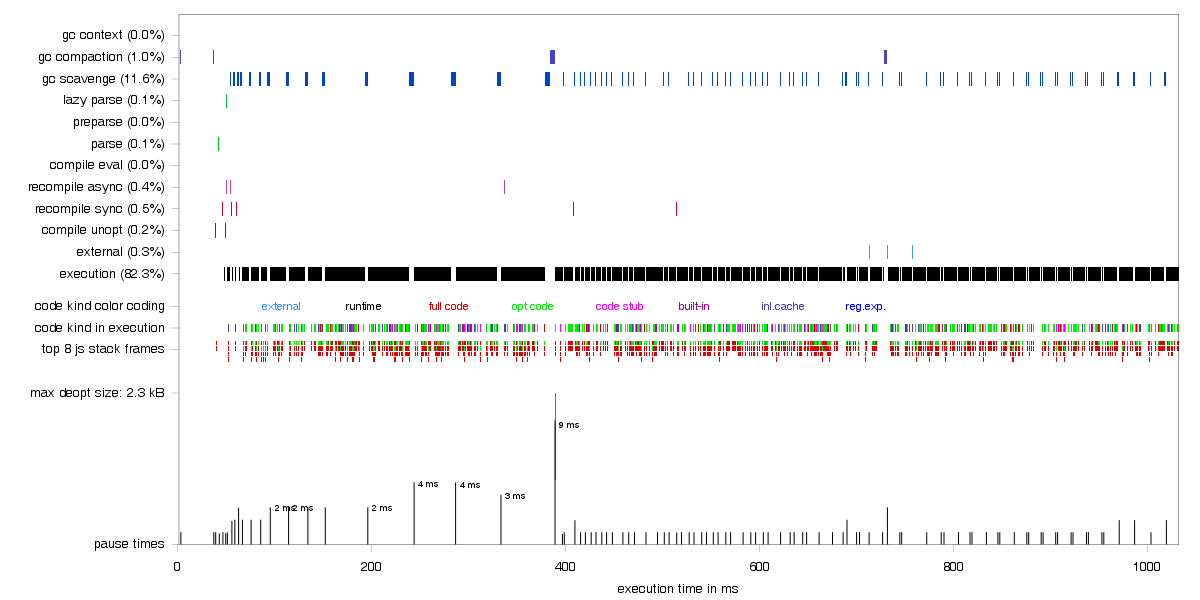
\includegraphics[width=16cm]{particles/particles1-profile.png}
\end{figure}

Garbage collection cycles blocking execution are also visible with --trace-gc flag.

\lstinputlisting[caption=Garbage collection in unoptimised particle system,label=listing:particles1gc]{particles/particles1gc.txt}

To improve performance different approach to particles allocation is used. Each particle has a flag "isDead" telling if it may be safely reused for new particle. Particle pool is kept along with a list of pointers to dead particles. This way when system reaches it's maximum congestion (around 15000 particles in given example) no new allocations occur.
Creation of new particles is moved from particle emitter to particle system, to avoid allocation of new array. Emitter works now as a structure describing behaviour but not implementing one.

\lstinputlisting[caption=Time measurement of optimized particle system in JavaScript,label=listing:timejs2]{particles/timejs2.txt}
\lstinputlisting[caption=Time measurement of optimized particle system in C++,label=listing:timecpp2]{particles/timecpp2.txt}

Optimised version shows overall improvement of 85\% for JavaScript and 45\% for C++ making JavaScript version only 2.2 times slower than native one. It's clearly visible that JavaScript is more sensitive to unwise memory management.

\lstinputlisting[caption=Profiler output for optimized particles,label=listing:particles1profile]{particles/particles2-profile.txt}

Profiling shows that step method of particle system now runs always in optimised mode and almost no time is spent on other methods. The same is visible on profiling chart, where "code kind in execution" stripe shows only optimised code.

\begin{figure}[h!]
  \caption{Chart of time used in optimised verion of JavaScript}
  \label{img:particles2profile}
  \centering
	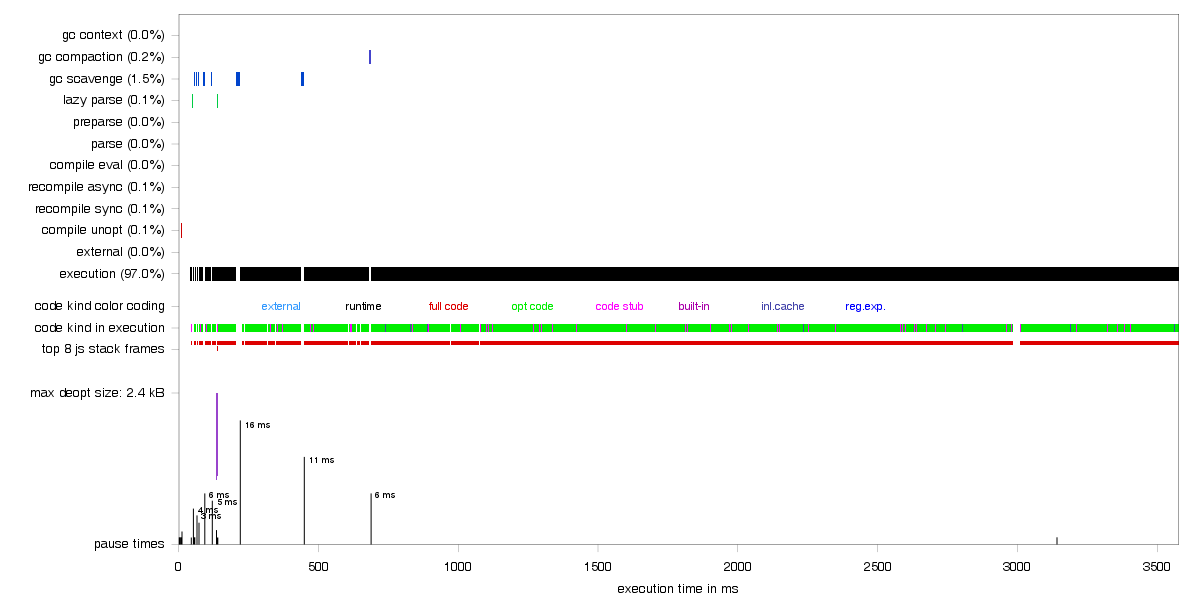
\includegraphics[width=16cm]{particles/particles2-profile.png}
\end{figure} 

Situation is also improved in garbage collection log.

\lstinputlisting[caption=Garbage collection in optimised particle system,label=listing:particles2gc]{particles/particles2gc.txt}
